\chapter{Algebra Features of CPSA}
\label{ch:algebra}

\index{Diffie-Hellman!algebra}
The {\cpsa} distribution comes equipped with two cryptographic
alegbras, the \texttt{basic} cryptoalgebra and the
\texttt{diffie-hellman} cryptoalgebra.  The Diffie-Hellman algebra is
a pure extension of the basic algebra, so a user may always use the
Diffie-Hellman algebra to access all algebraic features.  However, the
performance of the tool is superior when using the basic algebra, so
users are advised to choose the basic algebra whenever they are not
making use of Diffie-Hellman features.

In Chapter~\ref{ch:basic}, we introduced the basic cryptoalgebra,
along with the \texttt{data, text, name, skey,} and \texttt{akey}
sorts, and the \texttt{pubk, privk, invk, enc,} and \texttt{cat}
function symbols.  In addition to these, the basic cryptoalgebra
contains the sorts \ttindex{tag} \texttt{tag} and \texttt{mesg}, and the \texttt{ltk}
and \texttt{hash} function symbols, and string constants.

The Diffie-Hellman cryptoalgebra introduces three further sorts,
\texttt{base, rndx,} and \texttt{expt}, and six new function symbols,
\texttt{bltk, exp, rec, mul, gen,} and \texttt{one}.  For performance
reasons, one should always avoid using variables of sort
\texttt{base}.  Instead, replace the variable with \texttt{(exp (gen)
  x)}, where \texttt{x} is a variable of sort \texttt{expt}.

In this chapter we will explain these additional features with
examples.  In Section~\ref{sec:kerberos}, we will discuss the
\texttt{ltk} function symbol and the use of the \texttt{mesg} sort,
worked with an example based on the Kerberos protocol.  In
Section~\ref{sec:dh}, we will discuss the tool's Diffie-Hellman
features.  In Section~\ref{sec:other_algebra}, we will discuss the
remaining features, and note examples that demonstrate their use.
For a more complete reference about the two algebras, see Section~\ref{sec:algebra_ref}.

\section{Generic messages and long-term keys}
\label{sec:kerberos}

\index{Kerberos protocol}
\index{examples!Kerberos}
Securing communications purely with symmetric keys faces an inherent
scaling problem: when there are $n$ parties that may wish to
communicate, there must be $O(n^2)$ keys shared between parties, which
gets to be too many in any system with a large number of users.

The Kerberos protocol is a well-known protocol for the distribution of
symmetric keys.  Instead of having the $n$ parties share keys with
each other party, the users share a key only with a central key server
(also known as a key distribution center).  The key server controls
key distribution within a \emph{realm} that can be thought of as the
set of users that share keys with the key server.

Suppose a user wishes to communicate securely with another user in the
same realm.  The first user would contact the key server and request a
session key for communication with the other user.  The key server
could then encrypt the session key twice, once under each user's
shared key with the server.  One encrypted key is sent back to the
user that requested the channel, and the other (called the ``ticket'')
is also sent to the requesting user, to be forwarded on to their
communication partner.

We will focus on a flawed protocol similar to the initialization
protocol used by Kerberos.  The protocol is described informally as
follows.  There are three parties, the initiator $a$, the responder
$b$, and the key server $s$.

\begin{itemize}

\item $a$ sends a message $(a, b, n)$ to the key server, where $n$ is
  a freshly chosen nonce.

\item The key server, on a message $(a, b, n)$, picks a fresh, random
  session key $k$, and sends two encryptions to $a$:
  $\enc{k,n}{SK(a,s)}$ and $\enc{k,a,b}{SK(b,s)}$.  Here, $SK(x,s)$
  refers to the shared secret between the key server and~$x$.

\item $a$ receives these two messages, decrypts the first to learn $k$
  and to check that the proper nonce $n$ was included, then sends a
  message $m$ on to the responder, encrypted under $k$, along with the
  second message (the ticket).

\item $b$ receives two encrypted messages, decrypts the second to
  learn $k$, and decrypts the first with $k$ to learn the message.
\end{itemize}

\ttindex{ltk} The \texttt{ltk} function symbol is used in {\cpsa} to
represent long-term shared keys between two specific parties, when
communication of that key is assumed out of scope of the analysis.
See Figure~\ref{fig:kerb-flawed defprotocol} for a
\texttt{defprotocol} that attempts to describe this flawed version of
the Kerberos initialization protocol.  See \texttt{kerb.scm} in the
examples directory for the input file discussed here.

\begin{figure}
\centering
\begin{tabular}{l}
\verb|(defprotocol kerb-flawed basic|\\
\verb|  (defrole init|\\
\verb|    (vars (a b s name) (m n text) (k skey))|\\
\verb|    (trace (send (cat a b n))|\\
\verb|           (recv (cat (enc k n (ltk a s)) (enc k a b (ltk b s))))|\\
\verb|           (send (cat (enc m k) (enc k a b (ltk b s)))))|\\
\verb|    (uniq-orig n))|\\
\verb|  (defrole keyserv|\\
\verb|    (vars (a b s name) (n text) (k skey))|\\
\verb|    (trace (recv (cat a b n))|\\
\verb|           (send (cat (enc k n (ltk a s)) (enc k a b (ltk b s)))))|\\
\verb|    (uniq-orig k))|\\
\verb|  (defrole resp|\\
\verb|    (vars (a b s name) (m n text) (k skey))|\\
\verb|    (trace (recv (cat (enc m k) (enc k a b (ltk b s)))))))|\\
\end{tabular}
\caption{A flawed version of Kerberos}
\label{fig:kerb-flawed defprotocol}
\end{figure}

The actual Kerberos protocol contains several additional elements that
we omit for simplicity, but the key difference is that the message
encrypted under $SK(a,s)$ should include $b$.  The message from the
initiator that requests a session key is transmitted in the clear and
can be tampered with, so the initiator needs assurance that the
session key $k$ is being exposed only to the initiator and $b$.
Otherwise, even assuming the long-term keys of both $a$ and $b$ with
the key server are secure, a third party may observe the message $m$:
all the adversary has to do is block the initial message and substitute
$b$ with another name $c$.

Will {\cpsa} find this attack?  See \texttt{kerb.xhtml} for the
results of the analysis for the point-of-view skeleton described in
Figure~\ref{fig:kerb-flawed-pov}.  Note the use of
\texttt{defstrandmax}; this is a shortcut you can use in \cpsa to
specify a full-height instance of a role.

\begin{figure}
\centering
\begin{tabular}{l}
\verb|(defskeleton kerb-flawed|\\
\verb|  (vars (a b s name) (m text))|\\
\verb|  (defstrandmax init (a a) (b b) (s s) (m m))|\\
\verb|  (deflistener m)|\\
\verb|  (non-orig (ltk a s) (ltk b s))|\\
\verb|  (uniq-orig m))|\\
\end{tabular}
\caption{Flawed Kerberos point of view}
\label{fig:kerb-flawed-pov}
\end{figure}

Interestingly, the result of the analysis does not indicate any attack
is possible!  The analysis gets stuck at a skeleton (see
Figure~\ref{fig:kerb-skel4}) where the key server does in fact
generate a session key for $a$ and $b$, and where that session key is
exposed, but it cannot be exposed if it was generated for $a$ and $b$
and if we are assuming both of their long-term keys are private.

\begin{figure}
\centering
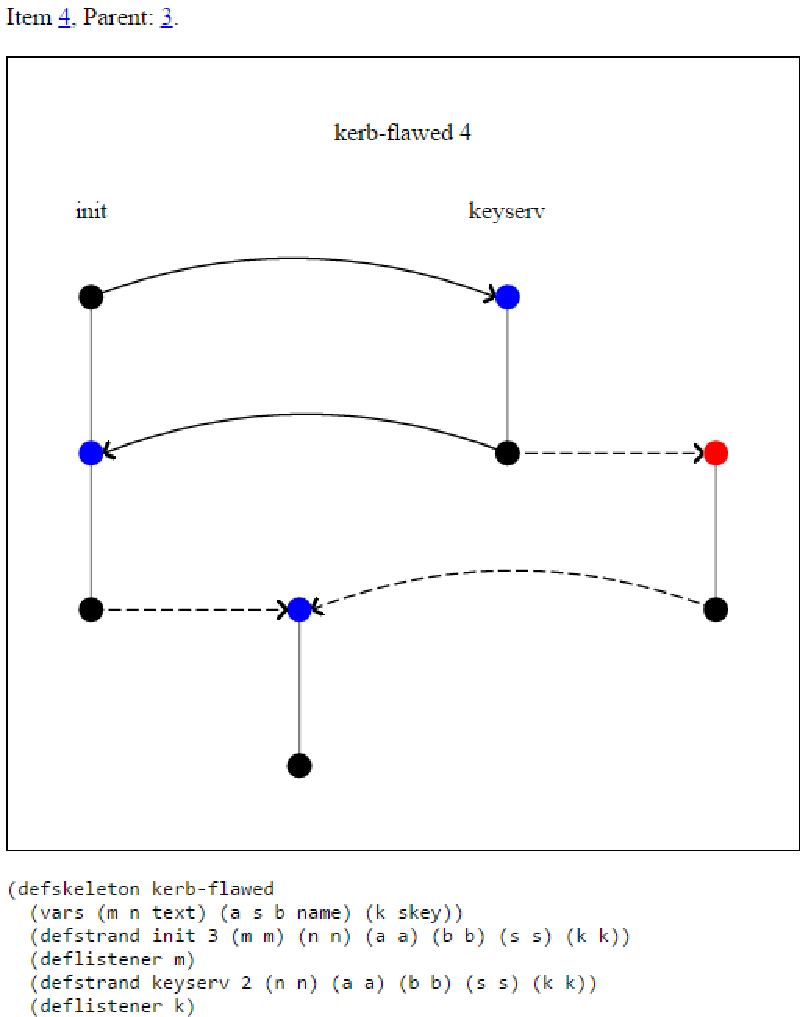
\includegraphics{kerb_skel4}
\caption[Flawed Kerberos dead skeleton]{Flawed Kerberos dead skeleton.  The use of the \texttt{mesg} sort provides a fix to this badly modeled version of the protocol.}
\label{fig:kerb-skel4}
\end{figure}

\ttindex{mesg} \index{generics} The reason {\cpsa} gets the wrong
result here is that we have inadvertently modeled our protocol
question incorrectly.  Specifically, we have described a version of
the protocol where the initiator is able to check the validity of the
ticket.  The attack we have in mind is one where the two encrypted
keys received by the initiator are prepared by a key server instance,
but one which does not agree with the initiator on $b$.  However, the
ticket would not match what the initiator expects in our expression of
the initiator role.\footnote{An alert reader may wonder how they could
  detect such an error of their own when using the tool.  We will
  return to this example in Chapter~\ref{ch:algorithm}, when we
  discuss how the {\cpsa} search process works.}

We described an initiator that will only proceed onto the third step
(sending $m$) if the ticket is of the form we specified.  In fact, the
initiator cannot do this.  The initiator cannot even verify that the
ticket is encrypted under the correct key! The solution is to use a
generic variable, one that can stand for any message, even one that a
particular participant cannot parse or understand.  The \texttt{mesg}
sort is the sort of all possible messages, so a variable of the
\texttt{mesg} sort can stand for any potential value at all.  See
Figure~\ref{fig:kerb-flawed2 defprotocol} for a version that models
the initiator's reception properly.  Note the \texttt{ticket} variable
in the initiator role, which stands for the ticket value the initiator
cannot inspect.

\begin{figure}
\begin{center}
\begin{tabular}{l}
\verb|(defprotocol kerb-flawed2 basic|\\
\verb|  (defrole init|\\
\verb|    (vars (a b s name) (m n text) (ticket mesg) (k skey))|\\
\verb|    (trace (send (cat a b n))|\\
\verb|           (recv (cat (enc k n (ltk a s)) ticket))|\\
\verb|           (send (cat (enc m k) ticket)))|\\
\verb|    (uniq-orig n))|\\
\verb|  (defrole keyserv|\\
\verb|    (vars (a b s name) (n text) (k skey))|\\
\verb|    (trace (recv (cat a b n))|\\
\verb|           (send (cat (enc k n (ltk a s)) (enc k a b (ltk b s)))))|\\
\verb|    (uniq-orig k))|\\
\verb|  (defrole resp|\\
\verb|    (vars (a b s name) (m n text) (k skey))|\\
\verb|    (trace (recv (cat (enc m k) (enc k a b (ltk b s)))))))|\\
\end{tabular}
\end{center}
\caption[Flawed Kerberos with a generic ticket]{Using a variable of
  sort \texttt{mesg} in a flawed version of Kerberos}
\label{fig:kerb-flawed2 defprotocol}
\end{figure}

This version of the flawed Kerberos protocol may also be found in the
file \texttt{kerb.scm}, and its analysis may be found in
\texttt{kerb.xhtml}.  This time, there is a shape found.  See
Figure~\ref{fig:kerb-skel7}.

\begin{figure}
\centering
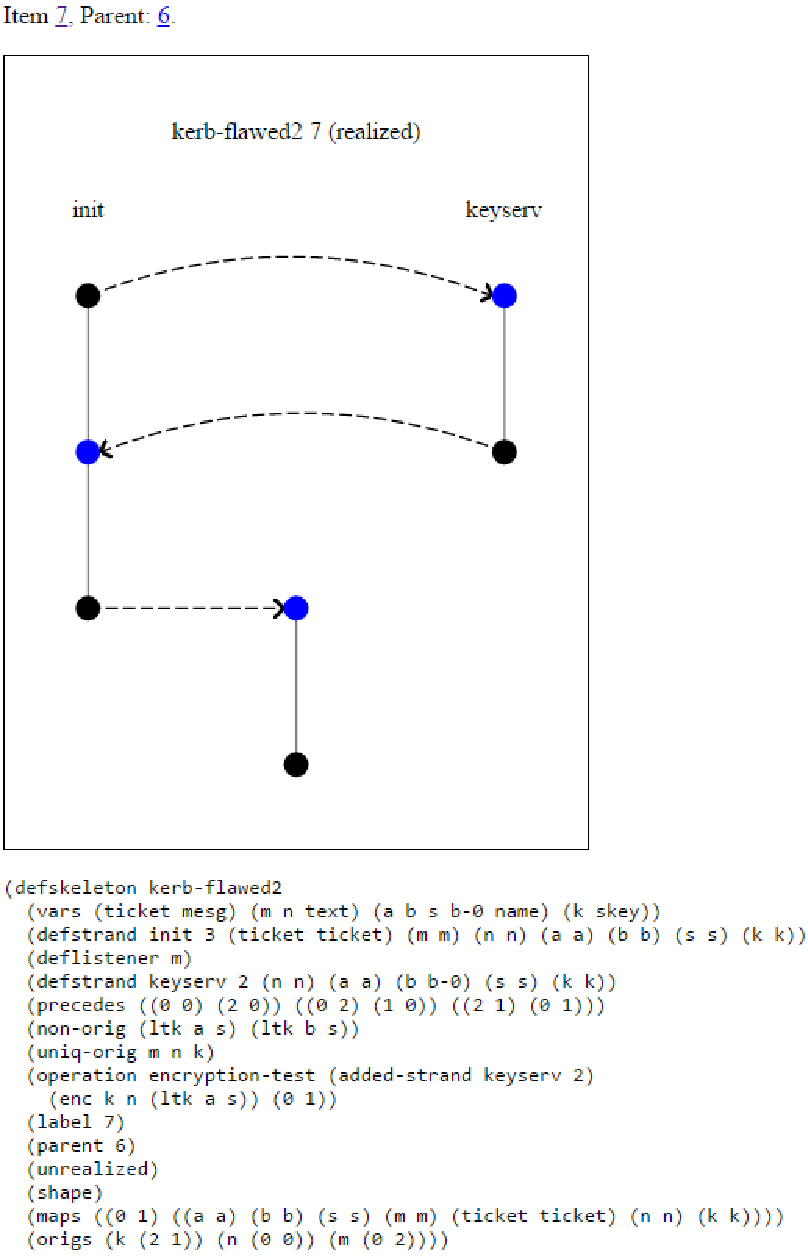
\includegraphics[scale=0.8]{kerb_skel7}
\caption[Flawed Kerberos shape]{Flawed Kerberos shape.  The use of the \texttt{mesg} variable allows us to find the attack illustrated here.}
\label{fig:kerb-skel7}
\end{figure}

\paragraph{Notes on generic variables.}
Variables of the \texttt{mesg} sort are constrained in {\cpsa}, and
may only be used when they are received before they are transmitted.
So for instance the $m$ variable in the initiator role of the flawed
Kerberos protocol cannot be of the \texttt{mesg} sort, because it
appears first in a transmission. However, if the responder is willing
to accept an encryption of any message $m$, then $m$ may declared as a
variable of the \texttt{mesg} sort within that role.

Also, variables of the \texttt{mesg} sort should never be used as a
key in any encryption.  This is because {\cpsa} uses a single function
symbol to represent both symmetric and asymmetric encryption, and when
the key is a variable of sort \texttt{mesg}, it is ambiguous which is
meant.

\paragraph{Notes on long-term keys.}
\ttindex{ltk}
Long-term keys are uni-directional: \texttt{(ltk a b)} and
\texttt{(ltk b a)} are distinct values.  In fact, {\cpsa} believes
that they cannot be the same unless $a = b$.  This is fine for
modeling protocols like Kerberos where there is a clear distinction
between client and server behavior.  Note that in our protocol
example, all long-term keys were described in all roles with a client
name in the first position and a server name in the second position.
See Section~\ref{sec:bltk} for discussion of the
\texttt{bltk} function symbol, which models \emph{bi-directional}
long-term symmetric keys.

\index{Yahalom protocol}\index{examples!Yahalom}
For another example of the use of long-term symmetric keys in a
protocol, see \texttt{yahalom.scm} in the examples directory.

\begin{exercise}
\label{ex:fix_kerberos}
Fix the flawed version of Kerberos so that the initiator can believe
their transmission is private to them and $b$.  Continue to use the
ticket variable of sort \texttt{mesg}.

Construct a \texttt{defskeleton} for the responder's point of view
for your fixed protocol, analyze it, and explain in English what
authentication property this analysis implies.
\end{exercise}

\begin{exercise}
  Construct a \texttt{defskeleton} for the initiator's point of view,
  without the listener for $m$, in the fixed version you created in
  Exercise~\ref{ex:fix_kerberos}.  Run the tool on your
  \texttt{defskeleton}.  Why are there dashed arrows in the result?
  Does this represent an insecurity in the protocol?

Whether or not you think this is an insecurity, think about how you
would alter the protocol to avoid the dashed arrows, and try out your
ideas.
\end{exercise}

\index{Otway-Rees protocol} \index{examples!Otway-Rees} The Otway-Rees
protocol is another example of very similar modeling; see
\texttt{or.scm} and \texttt{or.xhtml} if you wish to explore these
issues further on your own.

\section{Modeling Diffie-Hellman}
\label{sec:dh}

\index{Diffie-Hellman}
In their seminal 1976 paper, ``New Directions in Cryptography'',
Diffie and Hellman proposed the notion of public-key cryptography
\cite{DiffieHellman76}.  They did not have a method for public-key direct
encryption, but they did have a key exchange protocol that has become
a crucial building block in cryptographic protocols.

The Diffie-Hellman protocol works as follows.  A large prime number
$p$ is chosen and agreed upon as a parameter, and $g$ is chosen to be
some integer modulo $p$.  In order to enable secure communication
between arbitrary parties, Diffie and Hellman imagined a directory of
public values, like a phone book.  Each person who wishes to be able
to communicate securely with others will generate for themselves a
private value $x$, and publicize $g^x \bmod p$ as their public value.
If Alice's private value is $a$, and Bob's private value is $b$, then
the shared secret between Alice and Bob would be $g^{ab} \bmod p$,
which each party can calcuate from their own private value and their
partner's public value.  For instance, Alice can calculate $g^{ab}
\equiv (g^b)^a \bmod p$.

Version 3 of {\cpsa} introduces the Diffie-Hellman algebra, which
allows for analysis of protocols that incorporate Diffie-Hellman
techniques.  The Diffie-Hellman algebra includes all the function
symbols and sorts available in the basic algebra, plus three
additional sorts: two sorts (\texttt{rndx} and \texttt{expt}) for
exponents such as $x$, and \texttt{base}, for exponentiated values
such as $g^x$.  The Diffie-Hellman specific functions symbols are as
follows:

\begin{itemize}
\item \texttt{exp} represents exponentation.  For example, $h^x$ is
encoded as \\ \texttt{(exp h x)}.
\item \texttt{mul} represents multiplication of exponents.  So if $x$
is an exponent, \\ \texttt{(mul x x)} would represent the square of $x$.
\item \texttt{gen} represents the standard generator $g$.  It is
  probably best to think of \texttt{gen} as a constant, i.e. a
  function symbol with arity~0.

\item \texttt{one} represents the multiplicative identity for the group of
exponents.  Like \texttt{gen}, \texttt{one} is a 0-ary function.

{\bf Important: } \texttt{gen} and \texttt{one} are functions, so they
must be enclosed in parentheses.  So \texttt{(exp (gen) x)} represents
$g^x$, while \texttt{(exp gen x)} would represent ${gen}^x$ where
${gen}$ is expected to be a variable.  Similarly, \texttt{(mul (one)
  x)} represents $1 \cdot x$ while \texttt{(mul one x)} would
represent $one \cdot x$ where the tool expects $one$ to be an exponent
variable.

\item \texttt{rec} represents the multiplicative inverse in the group
  of exponents.  So for instance \texttt{(exp (exp (gen) x) (rec x)) =
    (exp (gen) (one)) = (gen)}.
\end{itemize}

At this time, {\cpsa} does not model addition of exponents, although
there are many examples of protocols that add or subtract exponents.
There is no way to take a product of exponentiated values either
(e.g. $g^x \cdot g^y$) since this would be equivalent to including
addition of exponents.

\index{Diffie-Hellman!unauthenticated}
\index{Diffie-Hellman!plain}
\index{examples!Diffie-Hellman}
Several examples of Diffie-Hellman protocols are available in the examples
directory of the distribution.  The \texttt{plaindh.scm} example models
a simple, unauthenticated Diffie-Hellman exchange between two parties.

The initiator and responder perform a Diffie-Hellman exchange, followed by
the initiator choosing a random nonce $n$ and sending it, encrypted with the
Diffie-Hellman key, to the responder, who decrypts $n$ and sends it back.

The analysis result can be found in \texttt{plaindh.xhtml}.  You can see
there that a shape is found where an initiator exists but no
responder; the $n$ can be decrypted because $g^{x x_0}$ can be
calculated by the adversary when $x_0$ is not assumed secret.

Two features of the {\cpsa} model of Diffie-Hellman in this protocol are
worth drawing attention to.  See Figure~\ref{fig:plaindh defprotocol}

\begin{figure}
\begin{center}
\begin{tabular}{l}
\verb|(defprotocol plaindh diffie-hellman|\\
\verb|  (defrole init|\\
\verb|    (vars (x rndx) (y expt) (n text))|\\
\verb|    (trace (send (exp (gen) x))|\\
\verb|           (recv (exp (gen) y)) |\\
\verb|           (send (enc n (exp (gen) (mul y x))))|\\
\verb|           (recv n))|\\
\verb|    (uniq-orig n)|\\
\verb|    (uniq-gen x))|\\
\verb| ...)|
\end{tabular}
\end{center}
\caption{Diffie-Hellman defprotocol}
\label{fig:plaindh defprotocol}
\end{figure}

\ttindex{rndx} \ttindex{expt}
Note that the initiator uses a variable $x$ of the \texttt{rndx} sort
to represent its own random variable, and a variable $y$ of the
\texttt{expt} sort to represent the exponent present in the base value
it receives from the initiator.  Distinct values of the \texttt{rndx}
sort model distinct independent random choices of exponents, while
\texttt{expt} values merely represent arbitrary exponents which may or
may not be calculated as some product of other known values.  Here,
since the initiator chooses their own exponent, we model $x$ as an
\texttt{rndx} value.  But since the initiator cannot know how the base value
$g^y$ was calculated, we model $y$ as an \texttt{expt} value.

Note that unlike the example in Section~\ref{sec:kerberos},
where receiving a specifically formatted encryption in a protocol role
implied the ability to decrypt and check that structure is present,
the use of a value like $g^y$ in a reception does not imply that $y$
is \emph{known}, only that $y$ is defined to be the value such that
$g^y$ is the base value received.

\ttindex{uniq-gen} Second, you may notice that $n$ is declared
\texttt{uniq-orig} while $x$ is declared \texttt{uniq-gen}.  The
difference between these declarations is rather technical: see
Section~\ref{sec:secrecy_assumptions} for details.  For the moment, it
is sufficient to say that one should use \texttt{uniq-gen} for
exponents that first occur within an exponentiation, rather than
\texttt{uniq-orig}.

\label{anchor:generalization}
\index{deletion} \index{generalization} It is also instructive to
examine the two final skeletons in the analysis that leads to the
shape; see Figure~\ref{fig:plaindh_skel4_5}.  The first realized
skeleton reached in the branch is skeleton 4, on the left, which
includes an instance of the initiator role and a listener.  But this
realized skeleton has a child: skeleton 5.  The difference is that
skeleton 5 does not include the listener.  This is an example of a
step that {\cpsa} takes called \emph{generalization}: when {\cpsa}
recognizes a realized skeleton (that is, one that has no unexplainable
receptions), it attempts to identify ways to make that skeleton more
general without losing coverage.  Here, {\cpsa} has deleted the
listener, because that actual explicit reception and re-transmission
of $g^{x x_0}$ is not strictly necessary.  When a realized skeleton
cannot be further generalized, {\cpsa} declares it a ``shape'' and
stops working in that branch of the analysis.

\begin{figure}
\centering
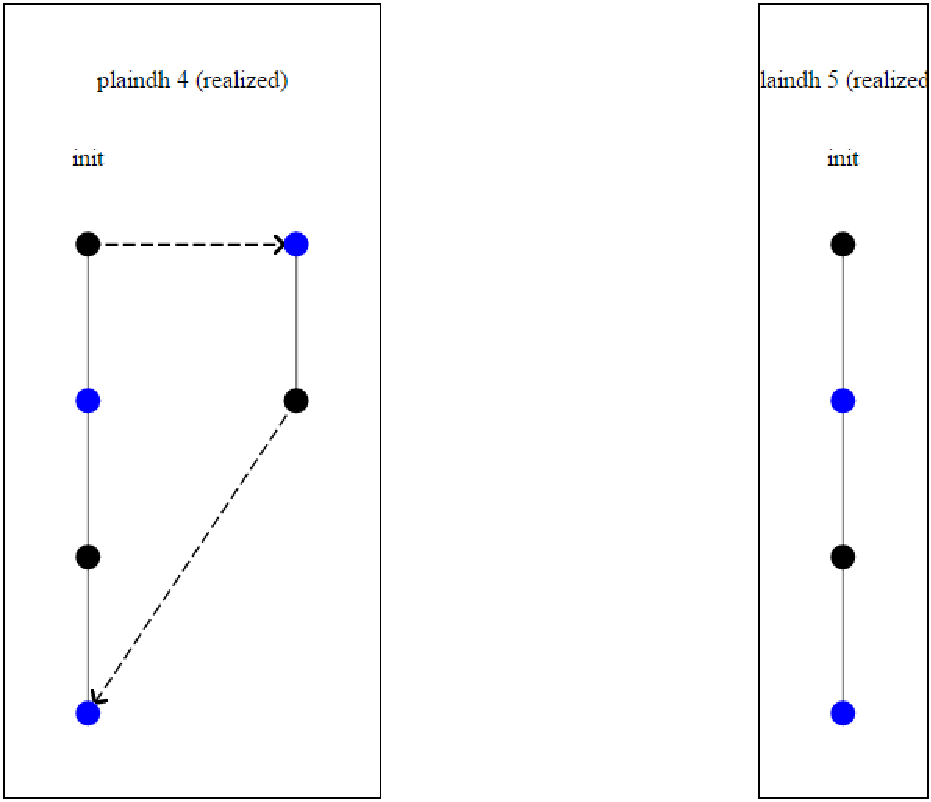
\includegraphics[scale=0.8]{plaindh_skel4_5}
\caption{Deletion of strand}
\label{fig:plaindh_skel4_5}
\end{figure}

\index{minimality of {\cpsa} output} You may notice there is another
shape in \texttt{plaindh.xhtml}, in which a responder is present.  As it
happens, the other shape is strictly less general than the shape shown
as skeleton 5.  {\cpsa} does not promise that the set of shapes it
outputs is strictly minimal, and this is one example where the output
of {\cpsa} is not minimal.

\subsection{Other examples}

\index{Station to Station protocol} \index{examples!Station to
  Station} The examples directory also contains the
\texttt{station.scm} and \texttt{station.xhtml} examples that model
the station-to-station protocol.  This protocol uses digital
signatures in order to authenticate a Diffie-Hellman exchange so that
the key established represents a secure and authenticated channel.
Two versions of the protocol are provided; in one, the Diffie-Hellman
exponents are assumed fresh in the roles, while in the other, they are
not.  The two analyses produce different results.

\index{forward secrecy}
\index{Unified Method} \index{examples!Unified Method} Another example
provided can be found in \texttt{iadh-um.scm} and
\texttt{iadh-um.xhtml}.  These inputs concern a method of determining
Diffie-Hellman session keys using both long-term and ``ephemeral''
exponents called the \emph{unified method}.  The ``ia'' in the example
name stands for \emph{implicitly authenticated}, because this method
of session key creation allows the parties to be sure that no other
party knows the key.  One interesting feature of this input is that it
contains an example of an exponent being transmitted outside of an
exponentiation.  Specifically, there is a role in which a party
generates and signs their long-term Diffie-Hellman public value, and
then compromises it by releasing the key.  The explicit compromise
allows us to test the ``forward secrecy'' property of the unified
method.

\section{Other Algebra Features}
\label{sec:other_algebra}

\subsection{Hashing}
\index{hash functions} \ttindex{hash} The {\cpsa} basic cryptoalgebra
includes a \texttt{hash} function symbol that can be used to represent
the use of a hash function.  The function takes a single input, but
\texttt{(hash t1 t2 ... tn)} is interpreted as shorthand for
\texttt{(hash (cat t1 (cat t2 ( \ldots tn) \ldots )))}.

\begin{exercise}
  The Needham-Schroeder protocol discussed in Chapter~\ref{ch:basic}
  was described as for key agreement, but no session key is apparent
  in the protocol.  The intention is to use the hash of the two nonces
  as the key.  Make a copy of the \texttt{ns.scm} example in which
  this key is explicitly used to encrypt and transmit a separate fresh
  value, and make a point of view testing the confidentiality of the
  plaintext.
\end{exercise}

\subsection{Constants}
\index{constants} \index{tags} \ttindex{tag} Numerous cryptographic
protocols make use of magic numbers or string constants to
disambiguate the purpose of various messages that occur during the
protocol.  {\cpsa} includes constant strings in the basic
cryptoalgebra.  Such constants always appear as quoted strings,
e.g. \texttt{"foo"}.  These strings do not need to be declared in a
\texttt{vars} statement because they are not variables.  Tags are
messages, so that a variable of
\verb|mesg| sort may be instantiated by a tag.

%   The sort of
%   string constants is always \texttt{tag}, which is a basic sort much
%   like \texttt{text} or \texttt{data}, however, it is strongly
%   recommended that the \texttt{tag} sort be used only for variables that
%   are intended to represent as-yet undetermined string constants.  See
%   Section~\ref{sec:distinct_decls} for strategies to avoid such
%   non-recommended uses.

\begin{exercise}
Note that in the Needham-Schroeder protocol, there seems to be no way
for an initiator to accidentally talk to another initiator, even though
the initiator both sends and receives an encrypted message with two
components in it.  Make a copy of the Needham-Schroeder protocol in which
the nonces are declared to be of sort \texttt{name} instead of \texttt{text},
so that $\enc{n_1,a}{K_b}$ and $\enc{n_1,n_2}{K_a}$ are modeled as similar
enough in format that confusing the two is possible.  What changes?

Then try adding distinct tag constants to each encrypted message, to
avoid the ambiguity we just created.  Run the analysis to see the
effect.
\end{exercise}

Constants may also be used to modify the \texttt{pubk} and
\texttt{privk} function symbols, to describe distinct keys associated
with a particular name.  For instance, one might use \texttt{(pubk
  "encrypt" a)} to describe the public encryption key of $a$, so as to
distinguish it from the public signature verification key of $a$.  Or,
one might wish to describe a certifying authority's
certificate-signing key but also a key used to sign certificate
revocation statements that might be different.

\subsection{Bidirectional Long-Term Keys}
\label{sec:bltk}
\ttindex{bltk}
\index{long-term key!bidirectional}
The \texttt{ltk} function symbol is used to describe the long-term secret
key shared between two parties.  However, the names of the two parties
are, in the function symbol, presented in a distinguished order.

In other words, {\cpsa} regards \texttt{(ltk a b)} and \texttt{(ltk b
  a)} as distinct from each other; in fact, they are only considered
equal when $a = b$.

The \texttt{bltk} function symbol is available in {\cpsa} in \emph{the
  Diffie-Hellman algebra only},\footnote{This choice may seem odd; it
  was made for performance reasons.  The presence of \texttt{bltk} or
  of Diffie-Hellman elements complicates some basic algebraic
  operations.  The \texttt{basic} cryptoalgebra is provided for
  optimized performance when analyzing protocols that do not include
  these features.} and regards the two names as equivalent in order.
In the Kerberos example discussed in Section~\ref{sec:kerberos}, we
noted that the server's name $s$ always appears second in our
\texttt{ltk} expressions.  This is fine if participants never can act
as both client and server, but if a participant can act as both, the
use of \texttt{ltk} implies that the participant maintains a strict
separation between the keys they share with other servers when acting
as a client (in which their own name appears first), and keys they
share with clients when acting as a server (in which their own name
appears second).

The use of \texttt{bltk} implies that participants can act as both
servers and clients, and that they only share one key with other
entities, and use that key both when acting as a server and when
acting as a client.

\index{Otway-Rees protocol!with bi-directional keys}
\index{examples!Otway-Rees!with bi-directional keys} See
\texttt{bltk\_or.scm} and \texttt{bltk\_or.xhtml} for modeling of the
Otway-Rees protocol with bi-directional long-term keys rather than
uni-directional ones.

\index{examples!Kerberos!with bi-directional keys}
\begin{exercise}
\label{ex:bltk_kerb}
Make a version of the flawed Kerberos input file \texttt{kerb.scm}
that uses bi-directional long-term keys instead.  Remember to switch
the algebra to Diffie-Hellman!  What differences do you observe?
\end{exercise}

\index{examples!Yahalom!with bi-directional keys}
\begin{exercise}
Repeat the Exercise~\ref{ex:bltk_kerb} but with the Yahalom protocol
(\texttt{yahalom.scm}) instead.
\end{exercise}

\section{The Lang Field:  Declaring new operators}
\label{sec:algebra:lang:field}

The signature of the message algebra used by {\cpsa} is extensible.
There are two forms of extensibility provided by {\cpsa}.  Users can
add operations for encryption, \index{tuple}tupling, and hashing; and
add sorts for atomic data.

A common extension is to add tupling operations to message algebras.
Previously, complex protocols often made use of tagged concatenation
to encode a tagged sequence of messages.  In {\cpsa}, concatenation is
implemented as sequences of pairing operations.  Thus, the expression
for a certificate body of the form
\begin{quote}
\begin{verbatim}
(cat "cert-body" dn serial-no pub-key)
\end{verbatim}
\end{quote}
is syntax for
\begin{quote}
\begin{verbatim}
(cat "cert-body" (cat dn (cat serial-no pub-key)))
\end{verbatim}
\end{quote}

Algebra extensions are declared using the \texttt{lang} key in the
protocol's association list, at the end of a protocol.  For the
certificate body example,
\begin{quote}
\begin{verbatim}
(defprotocol cert basic
  ...
  (lang (cert-body (tuple 3))))
\end{verbatim}
\end{quote}
adds one tupling operation so that the example above can be written as
\begin{quote}
\begin{verbatim}
(cert-body dn serial-no pub-key)
\end{verbatim}
\end{quote}
{\cpsa} represents this form internally as a sequence of messages with a
distinguished mark.  This representation is more efficient as compared
with the tagged concatenation representation.

\begin{table}
%\newcommand{\sym}[1]{\textup{\texttt{#1}}}
\begin{center}\scshape
\begin{tabular}{rcl}
  lang&$\leftarrow$&(\sym{lang} ldecl$\ast$)
  \\ ldecl&$\leftarrow$&(symbol+ kind)
  \\ kind&$\leftarrow$&
  $\sym{atom}\mid\sym{akey}\mid\sym{hash}\mid\mbox{(\sym{tuple}
    integer)}$
  \\ &$\mid$&$\sym{enc}\mid\sym{senc}\mid\sym{aenc}\mid\sym{sign}$
\end{tabular}
\end{center}
\caption{Lang Field Syntax}\label{tab:lang field syntax}
\end{table}

The syntax of a \index{lang field}\texttt{lang} declaration is given
in Table~\ref{tab:lang field syntax}.  There are eight kinds of ways
that {\cpsa} algebras can be extended.

\begin{itemize}

\item An atomic sort is added to the algebra when a symbol is declared
  to be of kind \texttt{atom}.  If \texttt{dollar} is declared to be
  an atomic sort, then \verb|(price dollar)| in a \texttt{var} form
  declares \texttt{price} to be of sort \texttt{dollar}.

\item An atomic sort is also added to the algebra when a symbol is declared
  to be of kind \texttt{akey}.  However, in addition to adding the
  sort, {\cpsa} adds the equation $(x^{-1})^{-1}=x$ for variables of
  the new sort.

\item A unary operation is added to the algebra when a symbol is
  declared to be of kind \texttt{hash}.  As with the default hash
  operation, the adversary cannot extract the contents of the hash.

\item An $n$-ary operation is added to the algebra when a symbol is
  declared to be of kind (\texttt{tuple} $n$).  As with concatenation,
 the adversary can construct and extract contents of tuples.
 Constraint: $n>0$.

\item A binary operation is added to the algebra when a symbol is
  declared to be of kind \texttt{enc}.  As with the default encryption
  operation, the adversary cannot extract contents of the encryption
  without access to the inverse of the key.

\item A symbol of kind \texttt{senc} is just like one of kind
  \texttt{enc} except that the key supplied when it is applied must be
  symmetric, that is, the sort of the key must not be asymmetric.

\item A symbol of kind \texttt{aenc} is just like one of kind
  \texttt{enc} except that the key supplied when it is applied must be
  asymmetric, but not the inverse applied to an asymmetric key.

\item A symbol of kind \texttt{sign} is just like one of kind
  \texttt{enc} except that the key supplied when it is applied must be
  the inverse applied to an asymmetric key.

\end{itemize}

%%% Local Variables:
%%% mode: latex
%%% TeX-master: "cpsa4manual"
%%% End:
